\documentclass[a4paper]{article}
\usepackage[utf8x]{inputenc}
\usepackage[T1,T2A]{fontenc}
\usepackage[russian]{babel}
\usepackage{hyperref}
\usepackage{indentfirst}
\usepackage{listings}
\usepackage{color}
\usepackage{here}
\usepackage{array}
\usepackage{multirow}
\usepackage{graphicx}
\setcounter{tocdepth}{3}

\usepackage{caption}
\renewcommand{\lstlistingname}{Программа} % заголовок листингов кода

\usepackage{listings}
\lstset{ %
extendedchars=\true,
keepspaces=true,
language=bash,					% choose the language of the code
basicstyle=\footnotesize,		% the size of the fonts that are used for the code
numbers=left,					% where to put the line-numbers
numberstyle=\footnotesize,		% the size of the fonts that are used for the line-numbers
stepnumber=1,					% the step between two line-numbers. If it is 1 each line will be numbered
numbersep=5pt,					% how far the line-numbers are from the code
backgroundcolor=\color{white},	% choose the background color. You must add \usepackage{color}
showspaces=false				% show spaces adding particular underscores
showstringspaces=false,			% underline spaces within strings
showtabs=false,					% show tabs within strings adding particular underscores
frame=single,           		% adds a frame around the code
tabsize=2,						% sets default tabsize to 2 spaces
captionpos=b,					% sets the caption-position to bottom
breaklines=true,				% sets automatic line breaking
breakatwhitespace=false,		% sets if automatic breaks should only happen at whitespace
escapeinside={\%*}{*)},			% if you want to add a comment within your code
postbreak=\raisebox{0ex}[0ex][0ex]{\ensuremath{\color{red}\hookrightarrow\space}}
}

\usepackage[left=2cm,right=2cm,
top=2cm,bottom=2cm,bindingoffset=0cm]{geometry}


\begin{document}	% начало документа

\begin{titlepage}	% начало титульной страницы

	\begin{center}		% выравнивание по центру

		\large Санкт-Петербургский Политехнический Университет Петра Великого\\
		\large Институт компьютерных наук и технологий \\
		\large Кафедра компьютерных систем и программных технологий\\[6cm]
		% название института, затем отступ 6см
		
		\huge Программирование\\[0.5cm] % название работы, затем отступ 0,5см
		\large Отчет по курсовой работе\\[0.1cm]
		\large Игра: Лабиринт\\[5cm]
	\end{center}


	\begin{flushright} % выравнивание по правому краю
		\begin{minipage}{0.25\textwidth} % врезка в половину ширины текста
			\begin{flushleft} % выровнять её содержимое по левому краю

				\large\textbf{Работу выполнил:}\\
				\large Мальцев М.С.\\
				\large {Группа:} 23501/4\\
				
				\large \textbf{Преподаватель:}\\
				\large Вылегжанина К.Д.

			\end{flushleft}
		\end{minipage}
	\end{flushright}
	
	\vfill % заполнить всё доступное ниже пространство

	\begin{center}
	\large Санкт-Петербург\\
	\large \the\year % вывести дату
	\end{center} % закончить выравнивание по центру

\thispagestyle{empty} % не нумеровать страницу
\end{titlepage} % конец титульной страницы

\vfill % заполнить всё доступное ниже пространство



% Содержание
\tableofcontents
\newpage



\section{Игровое приложение: Лабиринт}

Лабиринты – это одно их самых древних развлечений человечества. Еще в Древнем Риме добровольцы сами уходили в лабиринты, чтобы проверить свои выносливость и смекалку. К сожалению, многие не возвращались.\\

Лабиринт\footnote{https://en.wikipedia.org/wiki/Maze} — какая-либо структура (обычно в двухмерном или трёхмерном пространстве), состоящая из запутанных путей к выходу (и/или путей, ведущих в тупик).\\

Под лабиринтом у древних греков и римлян подразумевалось более или менее обширное пространство, состоящее из многочисленных залов, камер, дворов и переходов, расположенных по сложному и запутанному плану, с целью запутать и не дать выхода несведущему в плане лабиринта человеку.\\

Лабиринты всегда были слишком загадочным и заманчивым объектом, чтобы оказаться вне волшебного мира головоломок, но прежде чем стать популярной головоломкой, которая в наше время ассоциируется со словом "лабиринт" прошло не одно тысячелетие.\footnote{http://puzzlepedia.ru/historilabirint.html}\\

В современном мире головоломка лабиринт приобрела большую популярность. Можно с уверенностью утверждать, что данный тип головоломок повлиял на игровую индустрию, не только потому что существуют игры типа лабиринт, но и потому что множество приложений напрямую не относящиеся к данному игровому жанру включают себя лабиринты, например, Skyrim\footnote{https://ru.wikipedia.org/wiki/The\_Elder\_Scrolls\_V:\_Skyrim}\\

В связи со всем выше перечисленным, было принято решение создать игровое приложение, предоставляющее пользователю возможность прохождения лабиринтов.

\subsection{Концепция игрового приложения Лабиринт}

Программа представляет собой логическую игру, которая позволяет управлять существом помещённым в лабиринт.\\

Приложение отрисовывает игровое поле, на которе помещается существо. Пользователь может управлять им с помощью нажатия на то место, в которое он хочет переместить протагониста. Игра считается законченой, если пользователь довёл протагониста до выхода.
Для усложнения задачи прохождения существуют механизмы типа ключ-дверь(в некоторые ячейки игрового поля помещены двери, сквозь которые можно пройти только при наличие ключей).\\

\subsection{Задание}

Разработать приложение под операционные системы Windows 7+ и Android, позволяющее проходить лабиринты. 

\subsection{Минимально работоспособный продукт}

Приложение, которое предоставляет возможность пройти небольшой лабиринт.

\subsection{Вывод}

Пояснён выбор темы курсового проекта. Описана концепция игрового положения Лабиринт. Определено задание.

%#######################################################################################################

\section{Проектирование игрового приложения Лабиринт}

\subsection{Архитектура приложения}

Был использован шаблон проектирования Model-View-Presenter\footnote{https://ru.wikipedia.org/wiki/Model-View-Presenter}\\

Его использование обусловленно тем, что:

\begin{enumerate}  
\item[•]  требовалось обеспечить расширяемость приложения, так как существовала некоторая неопределённость по поводу того, какую функциональность должно предоставлять приложение, так как планировалось учесть новые пожелания пользователей
\item[•]  требовалось обеспечить скорость разработки
\item[•]  этот шаблон интересен с учебной точки зрения
\end{enumerate}

Был использован шаблон проектирования Observer\footnote{http://gameprogrammingpatterns.com/observer.html}. Целю его применения было оповещение слушателей о событиях окончания игры, открытия двери и нахождение игроком ключа.\\

Архитектура Модели выглядит следующим образом:
\begin{figure}[H]
	\begin{center}
		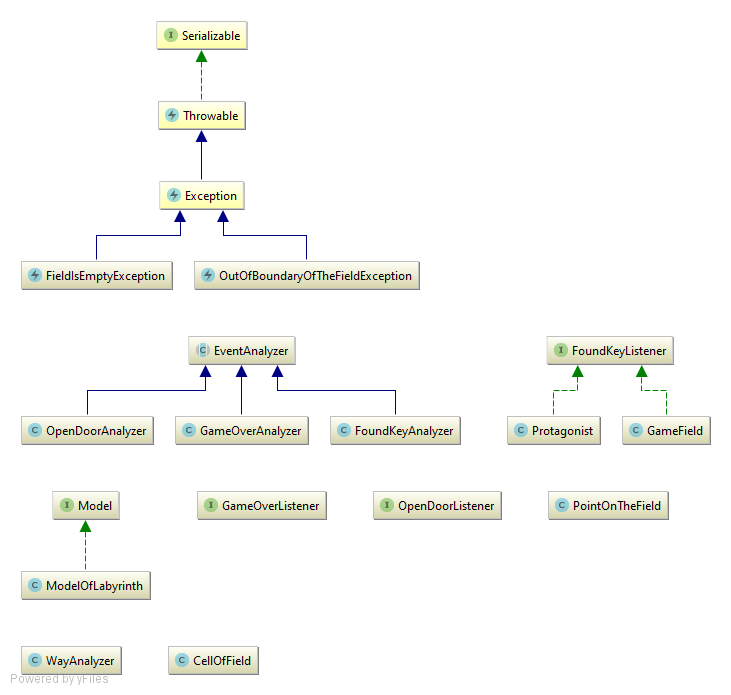
\includegraphics[scale=0.7]{pics/diagram.png}
		\caption{Диаграма классов Модели} 
		\label{pic:pic_name} % название для ссылок внутри кода
	\end{center}
\end{figure}

Модель предоставляет следующую функциональность:

\begin{enumerate}  
\item[•]  Получить список дверей на карте
\item[•]  Получить список ключей на карте
\item[•]  Получить позицию протагониста
\item[•]  Подписаться на события: окончания игры, открытия двери и нахождение игроком ключа, и отписаться от них
\item[•]  Передвинуть протагониста
\item[•]  Установить игровое поле
\item[•]  Получить проходимые ячейки поля
\item[•]  Получить информацию о проходимости ячейки
\end{enumerate}


\subsection{Диаграмма компонентов}

\begin{figure}[H]
	\begin{center}
		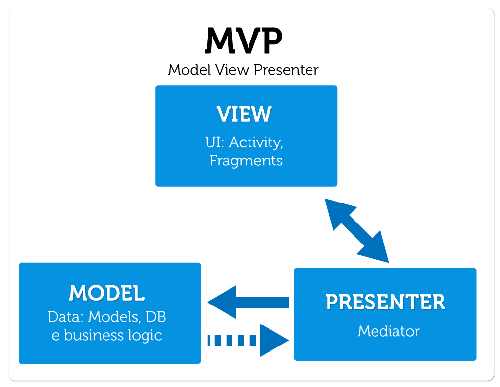
\includegraphics[scale=0.7]{pics/MVP-Process.png}
		\caption{Диаграмма компонентов} 
		\label{pic:pic_name} % название для ссылок внутри кода
	\end{center}
\end{figure}

\begin{enumerate}
\item[•] Модель -- содержит логическую часть игры, предоставляет данные для пользовательского интерфейса
\item[•] Представление -- отвечает за взаимодействие с пользователем путём отрисовки изображения на экране и фиксирования команд и событий, которы впоследствии перенаправляет Presenter'у
\item[•] Presenter -- управляет Моделью и Представлением. Указывает Представлению, что нужно отрисовывать в данный момент, принимает его оповещания о командах и сигнлах, реагирует на них и, если это необоходимо, связывается с Моделью для получения данных. 
\end{enumerate}

\subsection{Формат задания лабиринта}

Формат задания лабиринта: \\
\\
s00000\\
10k01f\\
101010\\
101010\\
111d10\\

Где:
\begin{enumerate}
\item[0] -- непроходимая ячейка поля
\item[1] -- проходимая ячейка поля
\item[s] -- это «start», начало пути
\item[f] -- это «finish», конец пути(выход)
\item[k] -- это «key», ключ 
\item[d] -- это «door», дверь
\end{enumerate}

Проходимых клеток должно быть минимум две, иначе этот лабиринт не будет использован.\\

Отсчёт координат ячеек ведётся с левой верхней.\\

Если не указать начало или конец пути, то они выбираются автоматически из проходимых клеток, соответственно первая и последняя, по номеру индекса.\\

Если передать лабиринт непрямоугольной формы, то он будет автоматически приведён к прямоугольнику путём отсечения лишних символов

\subsection{Вывод}

Было решено использовать шаблоны проектирования Model-View-Presenter и Observer. Была описана функциональность предоставляемая Моделью. Был объяснён формат задания лабиринтов.

\section{Реализация игрового приложения Лабиринт}

\subsection{Используемые версии}

\begin{enumerate}
\item[•]  IntelliJ IDEA 2016.3.1\\
Build IU-163.9166.29\\
For educational use only.\\
JRE: 1.8.0 102-b14 amd64\\
JVM: Java HotSpot(TM) 64-Bit Server VM by Oracle Corporation\\
\item[•]  Java language level: 6
\item[•]  Операционная система: Windows 10 x64
\item[•]  LibGDX 1.9.5
\item[•]  gdx-texturepacker-3.2.0
\item[•]  Система автоматической сборки: Gradle 2.14
\end{enumerate}

\subsection{LibGDX и его использование при разработке игрового приложения}

LibGDX\footnote{https://libgdx.badlogicgames.com} — фреймворк для создания игр и приложений, написанный на Java с использованием C и C++ (для более быстрой работы). Он позволяет писать кроссплатформенные игры и приложения используя один код. \footnote{https://ru.wikipedia.org/wiki/LibGDX}\\

Решение, о его использование было принято по трём причинам:
\begin{enumerate}
\item[1]  Кроссплатформенность, именно благодаря этому параметру была достигнута цель создать приложение сразу под две операционные системы
\item[2]  Удобство создания графических объектов
\item[3]  Фреймворк интересен с учебной точки зрения
\end{enumerate}



Большая часть его функциональных возможностей, описанных по ссылке\footnote{http://www.libgdx.ru/2013/08/introduction.html}, не использовалась, так как задача была максимально сузить его влияние на остальные части кода, помимо View. В итоге он не используется в Модели, а Presenter пользуется лишь пакетом com.badlogic.gdx.files, чтобы сделать чтение файла кроссплатформенным

\subsection{Процесс разработки игрового приложения}

Было проведено первичное знакомство с LibGDX и создано приложение, в котором почти не участвует Модель, но отображается протагонист на экране. После полученя опыта работы с LibGDX и принятия решения, что этот фреймворк подходит для решаемой задачи было решено заняться непосредственно развитием функциональности Модели. В итоге выбраный путь позволил корректировать Модель во время разработки таким образом, чтобы с ней было удобно работать, а UI в свою очередь позволил удобно использовать Модель.\\


На следующих изображениях поэтапно приведён процесс разработки приложения:

\begin{figure}[H]
	\begin{center}
		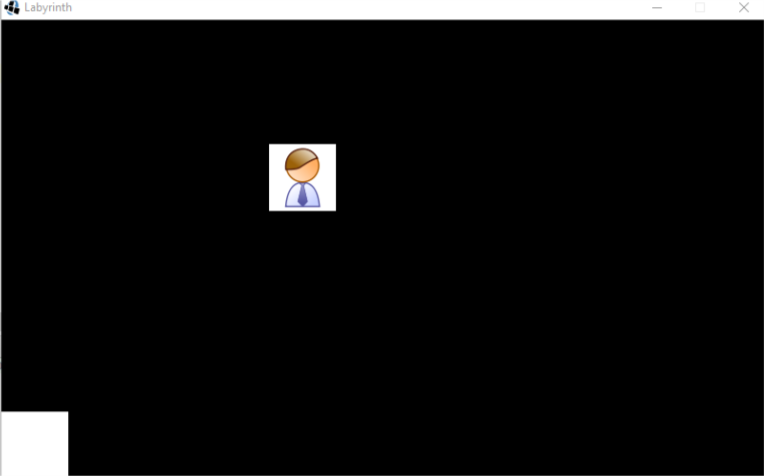
\includegraphics[scale=0.7]{pics/01.png}
		\caption{Снимок экрана иллюстрирующий вид пользовательского интерфейса на начальном этапе работы приложения} 
		\label{pic:pic_name} % название для ссылок внутри кода
	\end{center}
\end{figure}

На рисунке 3 изображён экран, на котором отрисовано изображение протагониста без участия Модели, поле, две белые клетки, которое задётся из Модели. Есть возможность перемещения героя между этими двумя клетками, в остальные части протагонист переместиться не может. 

\begin{figure}[H]
	\begin{center}
		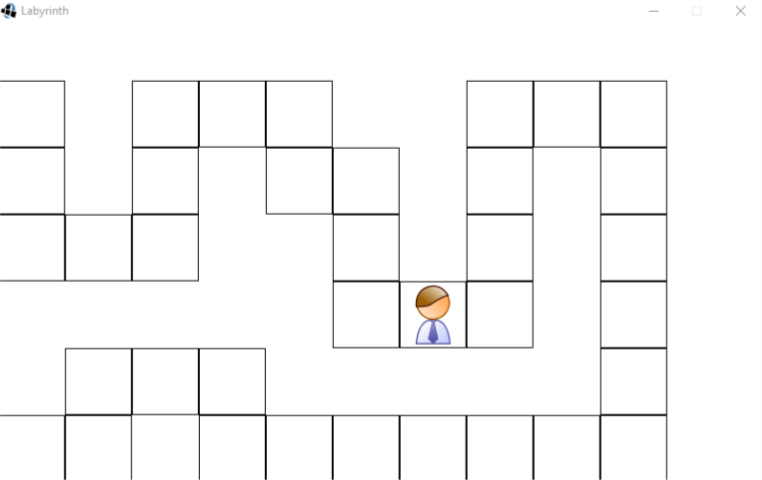
\includegraphics[scale=0.7]{pics/02.png}
		\caption{Снимок экрана иллюстрирующий вид пользовательского интерфейса после создания игрового поля} 
		\label{pic:pic_name} % название для ссылок внутри кода
	\end{center}
\end{figure}

На рисунке 4 в отличие от рисунка 3, поле задаётся путём передачи Модели определённого параметра. И было решено поменять цвет фона на белый. Протагонист может переместиться в любую проходимую точку поля.

\begin{figure}[H]
	\begin{center}
		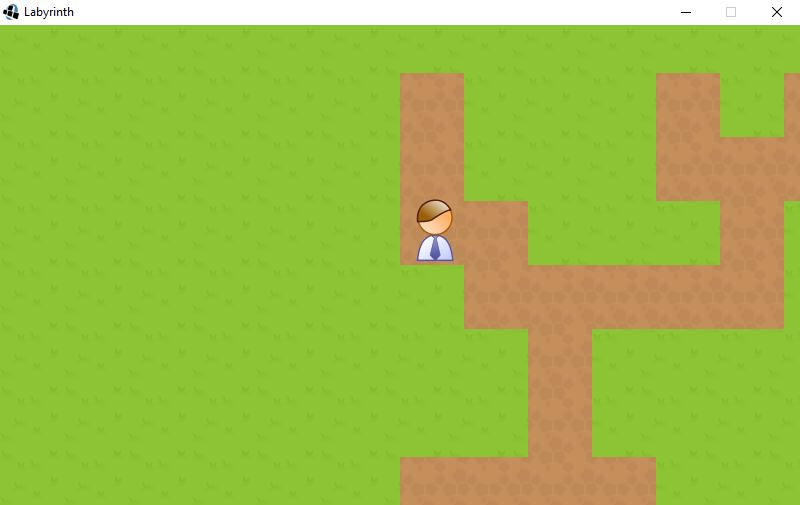
\includegraphics[scale=0.7]{pics/03.png}
		\caption{Наложение текстур} 
		\label{pic:pic_name} % название для ссылок внутри кода
	\end{center}
\end{figure}

Использовались текстуры с открытого источника\footnote{http://kenney.nl/assets}. 

\begin{figure}[H]
	\begin{center}
		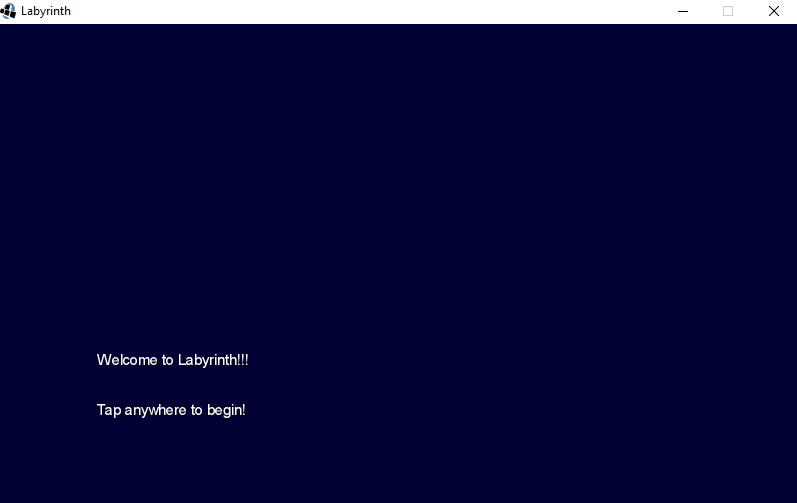
\includegraphics[scale=0.7]{pics/04.png}
		\caption{Добавление главного экрана} 
		\label{pic:pic_name} % название для ссылок внутри кода
	\end{center}
\end{figure}

Было решено добавить главный экран для приложения.

\begin{figure}[H]
	\begin{center}
		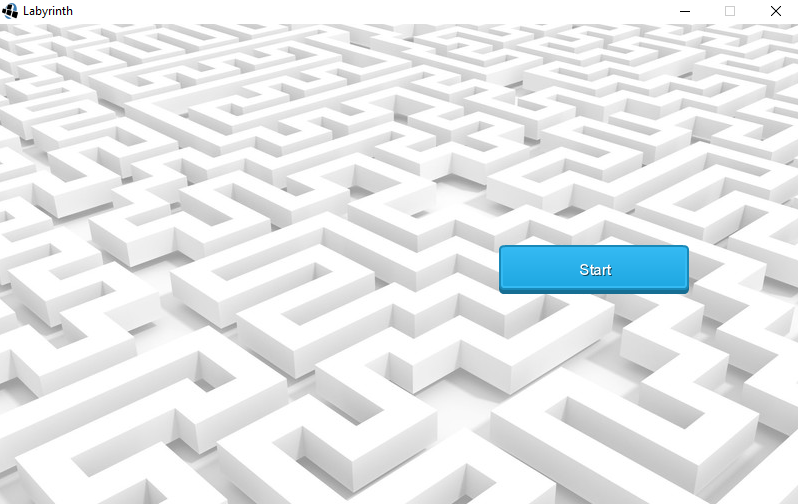
\includegraphics[scale=0.7]{pics/05.png}
		\caption{Декорирование главного экрана} 
		\label{pic:pic_name} % название для ссылок внутри кода
	\end{center}
\end{figure}

Оформление главного экрана было сделано с учётом тематики приложения.

\begin{figure}[H]
	\begin{center}
		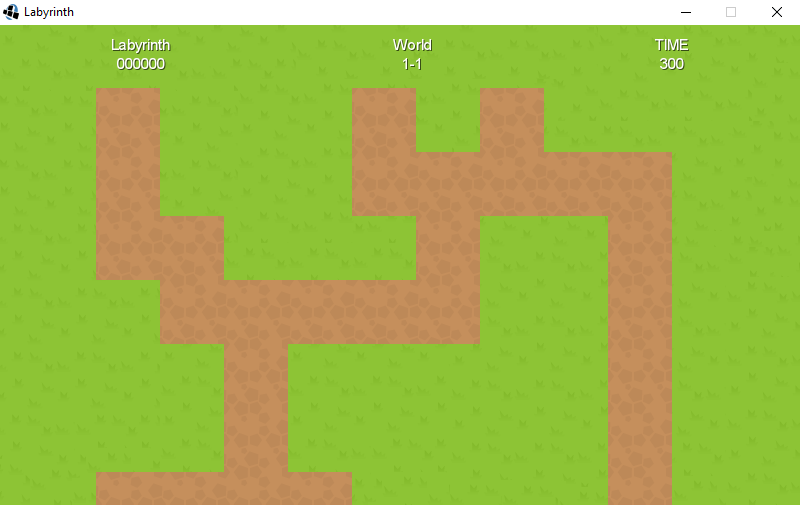
\includegraphics[scale=0.7]{pics/06.png}
		\caption{Добавление информационной панели} 
		\label{pic:pic_name} % название для ссылок внутри кода
	\end{center}
\end{figure}

Добавлена информационная панель, на которую выводится информация для пользователя.

\begin{figure}[H]
	\begin{center}
		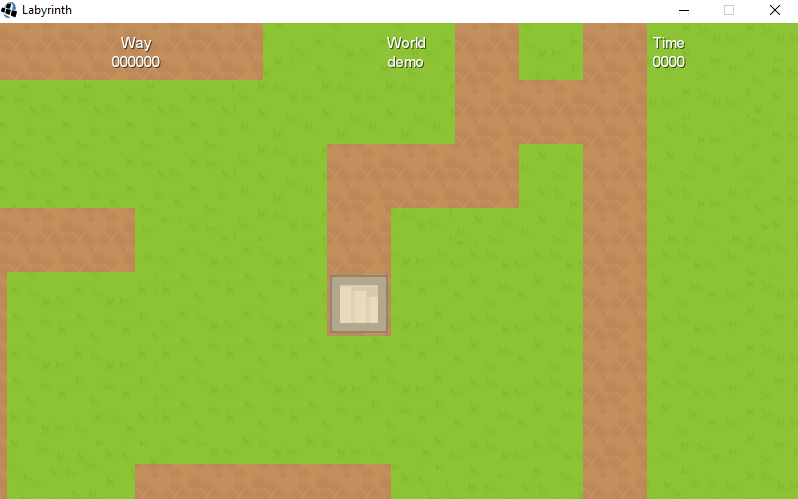
\includegraphics[scale=0.7]{pics/08.png}
		\caption{Обозначение выхода из лабиринта} 
		\label{pic:pic_name} % название для ссылок внутри кода
	\end{center}
\end{figure}

Выход из лабиринт обозначен специальной для него текстурой, которая была взята из уже упомянутого открытого ресурса.

\begin{figure}[H]
	\begin{center}
		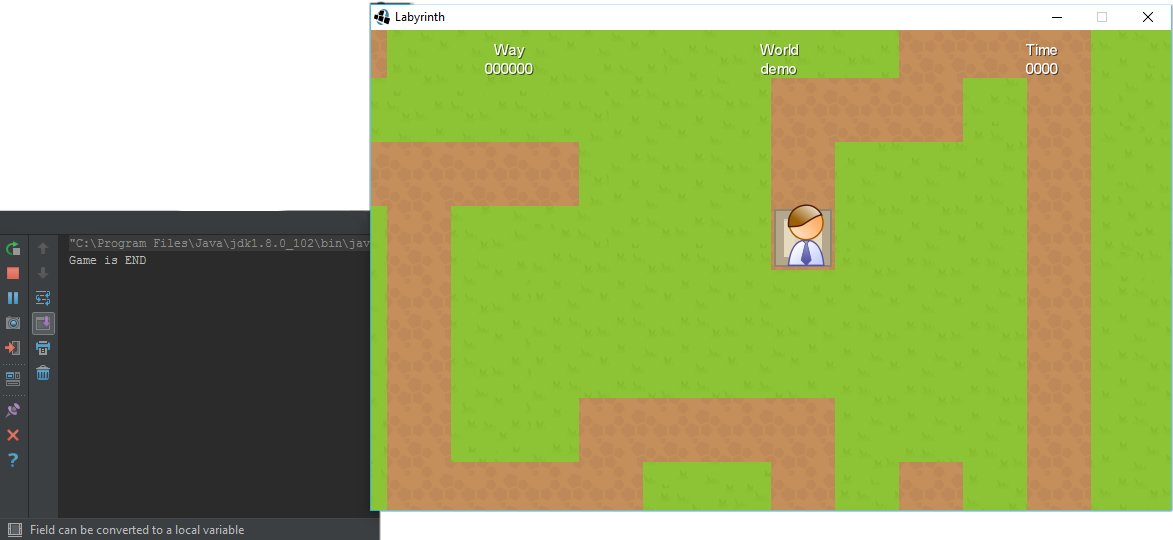
\includegraphics[scale=0.7]{pics/09.png}
		\caption{Реакция приложения на событие прохождение лабиринта} 
		\label{pic:pic_name} % название для ссылок внутри кода
	\end{center}
\end{figure}

На рисунке 10 изображён процесс реагирования приложение, на событие прохождение лабиринта. Протагонист помещён в ячейку поля, которая считается выходом из лабиринта, а приложение выводит в консоль сообщение о том, что игра окончена.


\begin{figure}[H]
	\begin{center}
		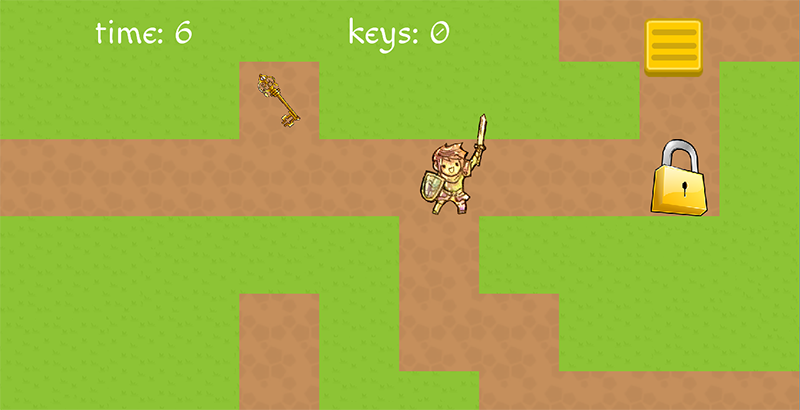
\includegraphics[scale=0.7]{pics/11.png}
		\caption{Окончательный вид игрового приложения} 
		\label{pic:pic_name} % название для ссылок внутри кода
	\end{center}
\end{figure}

В приложение были добавлены ключи и двери. В панель информации выводится время от начала игры, количество ключей, а так же там размещена кнопка выхода в главное меню приложения.

\subsection{Перспективы развития приложения}

Планируется реализовать следующую функциональность:
\begin{enumerate}
\item[•]  добавить миникарту, с отображением уже пройденого пути
\item[•]  добавить сюжетную линию
\item[•]  реализовать плавное перемещение протагониста, вместо перемещения рывками, в том числе и добавления анимации
\item[•]  и т.п.
\end{enumerate}

\subsection{Вывод}

Были описаны используемые средства разработки. Кратко описан фреймворк LibGDX и обосновано его использование. Был поэтапно описан процесс разработки приложения.

\section{Процесс обеспечения качества и тестирование игрового приложения Лабиринт}

\subsection{Просмотр кода}
Написаный код просматривался двумя людьми(Иван Крылов 16.12.2016 и ...) неучаствующими в его создании:
\begin{enumerate}
\item[•]  10 замечаний\footnote{https://github.com/mikle9997/Course-work/commit/fb61e9d6a3187a90e0aeacf34cb2c7dbcf346144}
\item[•]  143 замечания
\end{enumerate}

\subsection{Демонстрации}
Было проведено три демонстрации приложения\\

Во время демонстраций были высказаны следующие пожелания:
\begin{enumerate}
\item[1]  демонстрация: Начать писать логику приложения
\item[2]  демонстрация: Добавить ключи и двери
\item[3]  демонстрация: Поменять текстуры ключей и дверей, добавить выход из игрового процесса в главное меню
\end{enumerate}

\subsection{Автоматические тесты}

При разработке приложения были написаны автоматические тесты. Это значительно ускорило разработку приложения. С их помощью были выявленны такие ошибки как:

\begin{enumerate}
\item[•]  Неправильное построение пути между точками
\item[•]  Некорректная инициализация игрового поля
\item[•]  Проблемы добавления нового наблюдателя за событием и проблемы его оповещения
\item[•]  и т.п.\\
\end{enumerate}

Сценарий автоматических тестов, был следующий:
\begin{enumerate}
\item[1]  Создать экземпляр тестируемого класса
\item[2]  Поочереди проверить правильность работы всех механизмов класса, путём сравнивания с ожидаемым результатом
\item[3]  Проверить выводимый результат(информация, о том сколько тестов прошло, а сколько упало)
\item[4]  Радоваться, если всё хорошо или исправить упавшие тесты
\end{enumerate}

На изображении окно интегрированой среды разработки с результатами исполнения тестов

\begin{figure}[H]
	\begin{center}
		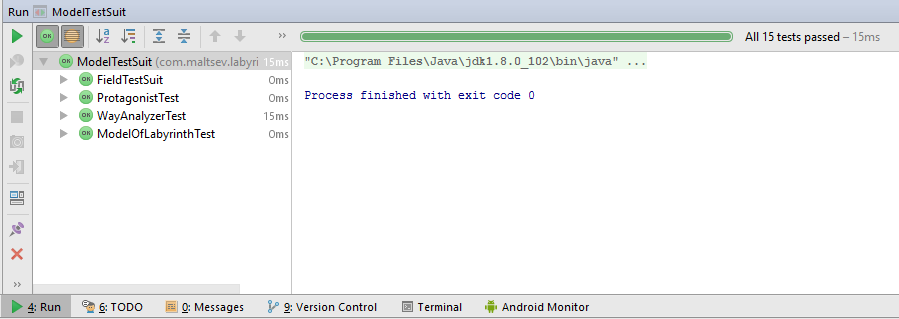
\includegraphics[scale=0.7]{pics/07.png}
		\caption{Процесс тестирования} 
		\label{pic:pic_name} % название для ссылок внутри кода
	\end{center}
\end{figure}

На следующих рисунках показан процент покрытия Модели тестами.

\begin{figure}[H]
	\begin{center}
		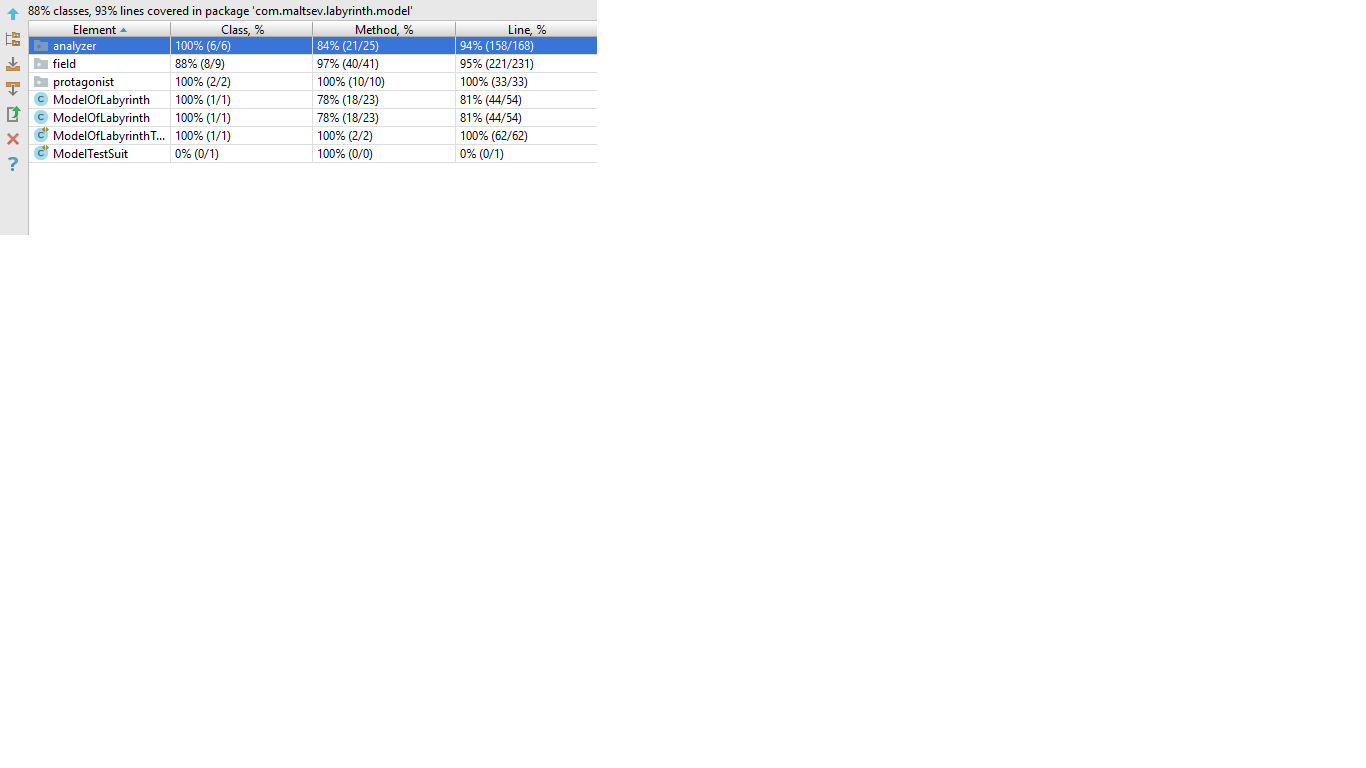
\includegraphics[scale=0.7]{pics/tests1.png}
		\caption{Таблица процентов покрытия кода для Модели} 
		\label{pic:pic_name} % название для ссылок внутри кода
	\end{center}
\end{figure}



\begin{figure}[H]
	\begin{center}
		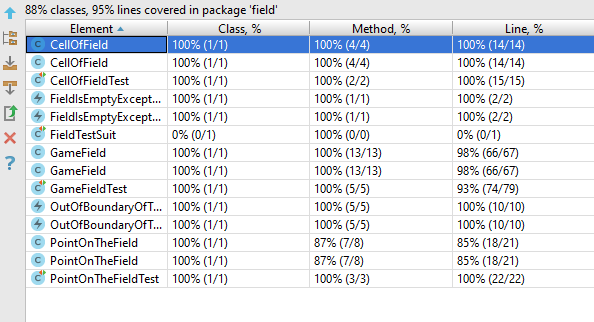
\includegraphics[scale=0.7]{pics/tests.png}
		\caption{Таблица процентов покрытия кода для пакета field из Модели} 
		\label{pic:pic_name} % название для ссылок внутри кода
	\end{center}
\end{figure}

Как показали тесты процент покрытия классов из Модели от 78-100\%

\subsection{Ручное тестирование}

Руками тестирование проводилось по следующему сценарию
\begin{enumerate}
\item[•]  Запустить приложение
\item[•]  Нажать на кнопку "Start" в главном меню
\item[•]  Нажать на точку, в которую мне хочется переместиться и проверить переместился ли протагонист туда
\item[•]  Собать ключ, путём помещения протагониста на клетку, с ключом и проверь отображение ключа в верхней панеле
\item[•]  Открыть дверь, путём помещения протагониста с ключом на клетку двери
\item[•]  Поместить протагониста на клетку выхода из лабиринта и проверить экран на появление панели выхода из игры
\item[•]  Проверить вышло ли приложение на главный экран
\item[•]  Сново нажать на конпку "Start"
\item[•]  Нажать на конпку выхода в меню и проверить вышло ли оно или нет
\end{enumerate}

\subsection{Нереализованая функциональность}

На данный момент:
\begin{enumerate}
\item[•]  останавливать таймер после конца игры
\item[•]  выводить результат таймера на панель конца игры
\item[•]  добавить спрайты изображений для плавности перехода
\item[•]  добавить экран паузы
\end{enumerate}

\subsection{Вывод}

Были описаны способы обеспечения качества и тестирования, а также описана нереализованая функциональность.

\section{Выводы}

Было разработано игровое приложение Лабиринт. Был изучен сторонний фреймворк LibGDX и патерн проектирования Model-View-Presenter. Созданое в ходе работы приложение было протестировано, также были определены возможные перспективы развития функциональности приложения. В дальнейшем планируется продолжение поддержки и улучшение приложения, а также исправление текущих недочётов.

\section{Приложение}

Исходный ход можно найти в репозитории\footnote{https://github.com/mikle9997/Course-work} на ресурсе GitHub

\subsection{Листинги}


\lstinputlisting{../Labyrinth/core/src/com/maltsev/labyrinth/model/Model.java}

\lstinputlisting{../Labyrinth/core/src/com/maltsev/labyrinth/model/ModelOfLabyrinth.java}

\lstinputlisting{../Labyrinth/core/src/com/maltsev/labyrinth/model/protagonist/Protagonist.java}

\lstinputlisting{../Labyrinth/core/src/com/maltsev/labyrinth/model/field/PointOnTheField.java}

\lstinputlisting{../Labyrinth/core/src/com/maltsev/labyrinth/model/field/OutOfBoundaryOfTheFieldException.java}

\lstinputlisting{../Labyrinth/core/src/com/maltsev/labyrinth/model/field/GameField.java}

\lstinputlisting{../Labyrinth/core/src/com/maltsev/labyrinth/model/field/FieldIsEmptyException.java}

\lstinputlisting{../Labyrinth/core/src/com/maltsev/labyrinth/model/field/CellOfField.java} 

\lstinputlisting{../Labyrinth/core/src/com/maltsev/labyrinth/model/analyzer/WayAnalyzer.java} 

\lstinputlisting{../Labyrinth/core/src/com/maltsev/labyrinth/model/analyzer/event/EventAnalyzer.java}

\lstinputlisting{../Labyrinth/core/src/com/maltsev/labyrinth/model/analyzer/event/gameover/GameOverAnalyzer.java}

\lstinputlisting{../Labyrinth/core/src/com/maltsev/labyrinth/model/analyzer/event/gameover/GameOverListener.java}

\lstinputlisting{../Labyrinth/core/src/com/maltsev/labyrinth/model/analyzer/event/keysanddoors/doors/OpenDoorAnalyzer.java}

\lstinputlisting{../Labyrinth/core/src/com/maltsev/labyrinth/model/analyzer/event/keysanddoors/doors/OpenDoorListener.java}

\lstinputlisting{../Labyrinth/core/src/com/maltsev/labyrinth/model/analyzer/event/keysanddoors/keys/FoundKeyAnalyzer.java}

\lstinputlisting{../Labyrinth/core/src/com/maltsev/labyrinth/model/analyzer/event/keysanddoors/keys/FoundKeyListener.java}

\lstinputlisting{../Labyrinth/core/src/com/maltsev/labyrinth/presenter/Presenter.java}

\lstinputlisting{../Labyrinth/core/src/com/maltsev/labyrinth/presenter/ParsingFile.java}

\lstinputlisting{../Labyrinth/core/src/com/maltsev/labyrinth/presenter/FileReader.java}

\lstinputlisting{../Labyrinth/core/src/com/maltsev/labyrinth/presenter/tempdata/PointOnTheScreen.java}

\lstinputlisting{../Labyrinth/core/src/com/maltsev/labyrinth/presenter/tempdata/SizeOfTexture.java}

\lstinputlisting{../Labyrinth/core/src/com/maltsev/labyrinth/presenter/interfaces/View.java}
 
\lstinputlisting{../Labyrinth/core/src/com/maltsev/labyrinth/view/Labyrinth.java}

\lstinputlisting{../Labyrinth/core/src/com/maltsev/labyrinth/view/screens/GameScreen.java}

\lstinputlisting{../Labyrinth/core/src/com/maltsev/labyrinth/view/screens/MainMenuScreen.java}

\lstinputlisting{../Labyrinth/core/src/com/maltsev/labyrinth/view/scenes/Fon.java}

\lstinputlisting{../Labyrinth/core/src/com/maltsev/labyrinth/view/scenes/Hud.java}

\end{document}
